% Copyright 2026 Sreeram Anil
% SPDX-License-Identifier: CC-BY-4.0
% =============================================================================
%  OCV-corrected Coulomb counting under light load — baseline family
% =============================================================================
\chapter{OCV-Corrected Coulomb Counting (Hybrid)}
\label{ch:coulombocvhybrid}

\section*{At a glance}
\begin{tabular}{@{}l>{\raggedright\arraybackslash}p{0.76\textwidth}@{}}
Family & baselines \\
Header & \texttt{include/estkit/battery/baselines.hpp} \\
Registered name & \texttt{CoulombOCVHybrid} \\
State dimension & $n_x = 4$ propagated open-loop; $\soc$ corrected while $\abs{i} < 0.3\,$C \\
Options & \code{i\_thr\_C} $=0.3$, \code{tau\_corr} $=\SI{60}{\second}$ \\
Cost per step & $\mathcal{O}(n_x)$ under load, $+\,n_b=40$ bisection steps when correcting; $\approx 211$\,ns/step \\
Primary references & \cite{ng2009coulomb,plett2015bms1,hu2012comparative} \\
\end{tabular}

\section{Motivation and relevance}
Chapters~\ref{ch:coulombcounting} and~\ref{ch:ocvlookup} established a clean complementarity.
Ampere-hour integration is smooth, cheap and drift-prone, and its error
\eqref{eq:cc-drift} grows without bound. Open-circuit-voltage inversion is bounded and
memoryless, but under load its accuracy is set by how well the overpotential
$R_0 i + v_1 + v_2 - Mh$ --- several hundred millivolts during a hover --- is modelled, and the
low-pass it needs to reject noise converts the SOC rate into a lag of
\SI{3.75}{\percent} \eqref{eq:ocv-lag}.

Both objections to the voltage inversion vanish at \emph{low current}: the overpotential to be
compensated shrinks in proportion to $i$, so a \SI{10}{\percent} error in $R_0$ costs
\SI{1.2}{\milli\volt} at \SI{1}{\ampere} instead of \SI{27}{\milli\volt} at \SI{22.5}{\ampere}, and
the lag term $\tau i/(3600Q)$ shrinks with it. The engineering response --- and what most shipped
battery-management systems implement in one form or another --- is therefore to integrate at all
times and to \emph{pull the count towards the voltage-derived SOC whenever the load is light enough
for that SOC to be trustworthy}: the cheapest possible approximation to a Kalman filter, a gain that
is zero above a current threshold and a fixed first-order constant below it, scheduled on the
measured current instead of computed from a covariance.

The interest for an electric aircraft is that this is the only baseline that is both drift-corrected
\emph{and} usable in flight. It does not require the cell to rest --- an eVTOL mission contains no
rest at all --- only that the mission contain phases at a fraction of the cruise current, which
preflight checks and postflight shutdown do provide: about \SI{10}{\percent} of every profile in the
benchmark (\S\ref{sec:hy-duty}).

\section{Problem statement}
The method estimates $\soc$ by \eqref{eq:cc-recursion} and applies a correction whenever the
measured current is below a threshold.
\begin{assumption}\label{as:hy-all}
(i) Below $i_{\text{thr}}$, the compensated open-circuit voltage \eqref{eq:ocv-compensate} is an
unbiased proxy for $\ocv(\soc,T)$ --- that is, the residual model error at low current is small
compared with the accuracy required; (ii) the mission contains enough time below $i_{\text{thr}}$
for a first-order correction of time constant $\tau_{\text{corr}}$ to act.
\end{assumption}
Assumption~(i) fails for the hysteresis, which does \emph{not} shrink with current, and for the
SPM plant at low temperature; assumption~(ii) is a property of the duty cycle, quantified in
\S\ref{sec:hy-duty}.

\section{Derivation}

\subsection{The blended update}
Each sample performs the open-loop time update of the full four-state model --- Coulomb counting on
$\soc$, and the RC and hysteresis states driven by the measured current --- and then, conditionally,
a correction on $\soc$ alone:
\begin{align}
\xhat_k &= f(\xhat_{k-1}, \vu_{k-1}), \label{eq:hy-predict}\\
\widehat{\ocv}_k &= v^{\text{m}}_k + R_0(T^{\text{m}}_k)\,i^{\text{m}}_k
 + \hat v_{1,k} + \hat v_{2,k} - M\,\hat h_k, \label{eq:hy-proxy}\\
\hat\soc_k &\gets a\,\hat\soc_k + (1-a)\,\ocv^{-1}\!\bigl(\widehat{\ocv}_k, T^{\text{m}}_k\bigr),
 \qquad a = e^{-\dt/\tau_{\text{corr}}},
 \qquad\text{if } \abs{i^{\text{m}}_k} < i_{\text{thr}}, \label{eq:hy-correct}
\end{align}
with $i_{\text{thr}} = 0.3\,Q_{\text{nom}}/\si{\hour} = \SI{1.5}{\ampere}$ for the
\SI{5}{\ampere\hour} cell and $\tau_{\text{corr}} = \SI{60}{\second}$, so
$a = e^{-0.1/60} = 0.998334$. The inversion $\ocv^{-1}$ is the same 40-step bisection on
$[-0.05,1.05]$ used in Chapter~\ref{ch:ocvlookup}; the compensation \eqref{eq:hy-proxy} is
also identical, so the method is exactly ``Coulomb counting, dragged towards \code{OCVLookup}'s
instantaneous estimate at a rate $1/\tau_{\text{corr}}$, but only while the load is light''.

Two structural points distinguish it from the rest-based re-anchoring of ground-vehicle practice: it
never waits (there is no rest timer and no dwell, so the correction begins on the first light-load
sample), and the RC states are \emph{compensated} rather than assumed decayed, so the
overpotentials need not be zero --- only small enough that the model's error in them is tolerable.

\subsection{Error dynamics}
Let $e_k = \hat\soc_k - \soc_k$ and let $e^{\ocv}$ denote the error of the voltage-derived SOC
itself, which by \eqref{eq:ocv-error} is the compensated-voltage error divided by the OCV slope.
Combining \eqref{eq:cc-drift} with \eqref{eq:hy-correct}, the error obeys a \emph{switched} linear
recursion: in continuous-time form,
\begin{equation}
\dot e \;=\;
\begin{cases}
\;\;\dot e_{\text{drift}}, & \abs{i} \ge i_{\text{thr}} \quad\text{(open loop)},\\[4pt]
-\dfrac{1}{\tau_{\text{corr}}}\bigl(e - e^{\ocv}\bigr) \;+\; \dot e_{\text{drift}},
 & \abs{i} < i_{\text{thr}} \quad\text{(corrected)},
\end{cases}
\label{eq:hy-switched}
\end{equation}
where $\dot e_{\text{drift}}$ is the instantaneous version of the gain, offset and capacity terms of
\eqref{eq:cc-drift}. Over a single light-load window $[t_0,t_1]$ of duration $T_w$, and neglecting
the drift accumulated within it (at $\abs{i}<\SI{1.5}{\ampere}$ it is at most
\SI{0.02}{\percent} of SOC per minute), \eqref{eq:hy-switched} integrates to
\begin{equation}
\boxed{\;
e(t_1) \;=\; e^{\ocv} \;+\; \bigl(e(t_0) - e^{\ocv}\bigr)\,e^{-T_w/\tau_{\text{corr}}} \;}
\label{eq:hy-window}
\end{equation}
so each light-load window contracts whatever error the estimator is carrying by the factor
$e^{-T_w/\tau_{\text{corr}}}$, towards a floor $e^{\ocv}$ that the correction cannot go below.
Three consequences follow, and between them they explain every row of the results table.

\paragraph{The error is reduced, never removed, and only in bursts.} An initial error survives a
mission in proportion to the \emph{total} light-load time: with windows $T_{w,1},T_{w,2},\dots$ the
surviving fraction is $\exp\bigl(-\sum_j T_{w,j}/\tau_{\text{corr}}\bigr)$. Between windows the
estimate is pure Coulomb counting and the error is frozen at whatever the last window left. This is
visible as a staircase in the error trace and is the defining signature of the method.

\paragraph{The floor is the low-current OCV error.} $e^{\ocv}$ is what
Chapter~\ref{ch:ocvlookup} measures, evaluated at $\abs{i}<i_{\text{thr}}$ rather than at the hover
current, and with a much smaller lag: $\tau_{\text{corr}}\,i/(3600Q) = \SI{0.33}{\percent}$ at
\SI{1}{\ampere} against \SI{3.75}{\percent} for \code{OCVLookup} at hover. The two terms of
\eqref{eq:ocv-error} that do \emph{not} shrink with current are the voltage-sensor error and the
hysteresis mismatch $M\,\delta h$, and the latter therefore sets the floor: with
$M = \SI{5}{\milli\volt}$ and an estimator that initialises $\hat h_0 = 0$ while the plant arrives
from a charge at $h=+1$, the proxy is biased by \SI{5}{\milli\volt}, i.e.\
$5/800 = \SI{0.6}{\percent}$ of SOC at mid-slope.

\paragraph{The threshold is a duty-cycle decision, not a tuning knob.} $i_{\text{thr}}$ decides
which mission segments contribute at all, and because a profile is a staircase in current, the map
from $i_{\text{thr}}$ to correction time is a step function.

\subsection{How much light load does a mission contain?}
\label{sec:hy-duty}
Counting the samples with $\abs{i^{\text{m}}}<\SI{1.5}{\ampere}$ in each benchmark profile
(seed~1, nominal sensors) gives:

\begin{table}[H]\centering\small
\caption{Light-load duty of the benchmark profiles at $i_{\text{thr}} = 0.3\,$C
($\SI{1.5}{\ampere}$), and the resulting contraction factor
$\exp(-\sum T_w/\tau_{\text{corr}})$ applied to any error the estimator carries into the mission.}
\label{tab:hy-duty}
\begin{tabular}{@{}lrrrr@{}}\toprule
profile & mission [\si{\second}] & light load [\si{\second}] & fraction & $\sum T_w/\tau_{\text{corr}}$ \\ \midrule
\code{evtol}          & 2010 & 210.0 & \SI{10.4}{\percent} & 3.50 \\
\code{fixed\_wing}    & 2880 & 331.6 & \SI{11.5}{\percent} & 5.53 \\
\code{hover\_hold}    & 1140 & 120.0 & \SI{10.5}{\percent} & 2.00 \\
\code{ground\_charge} & 3600 & 526.0 & \SI{14.6}{\percent} & 8.77 \\
\bottomrule\end{tabular}
\end{table}

For the eVTOL mission the light-load time is exactly the \SI{120}{\second} \code{preflight} and the
\SI{90}{\second} \code{postflight} segments, both at 0.20\,C $=\SI{1.0}{\ampere}$; \code{taxi} at
0.50\,C $=\SI{2.5}{\ampere}$ is excluded, and so is everything else. The threshold choice is what
makes those two segments count: at $i_{\text{thr}} = 0.2\,$C nothing in the mission would qualify,
and at $0.55\,$C the two taxi segments would be added. \code{fixed\_wing} is the interesting case:
its \code{descent} segment sits at exactly 0.30\,C, so with a \SI{15}{\percent} gust fraction it
straddles the threshold and contributes about \SI{150}{\second} of intermittent, chattering
correction --- a reminder that a hard threshold on a noisy signal is a switching surface, and that a
production implementation should hysteresis-band it.

\section{Algorithm}
\begin{algorithm}[H]
\caption{OCV-corrected Coulomb counting --- one sampling period}
\begin{algorithmic}[1]
\Require $\xhat_{k-1}$, stored $\vu_{k-1}$, new $i^{\text{m}}_k, v^{\text{m}}_k, T^{\text{m}}_k$
\State $\vu_k \gets [\,i^{\text{m}}_k,\ T^{\text{m}}_k\,]^\T$
\If{$k>0$} \State $\xhat_k \gets f(\xhat_{k-1},\vu_{k-1})$ \Comment{ampere-hour integration plus open-loop $v_1,v_2,h$}
\EndIf
\State $\hat v_k \gets h(\xhat_k,\vu_k)$ \Comment{prior voltage prediction, for the residual metric}
\If{$\abs{i^{\text{m}}_k} < i_{\text{thr}}$}
 \State $\widehat{\ocv} \gets v^{\text{m}}_k + R_0(T^{\text{m}}_k)\,i^{\text{m}}_k + \hat v_1 + \hat v_2 - M\hat h$
 \State $\soc^{\ocv} \gets$ \textbf{bisect} $\ocv(\cdot,T^{\text{m}}_k) = \widehat{\ocv}$ on $[-0.05,1.05]$, 40 steps
 \State $\xhat_k[\soc] \gets a\,\xhat_k[\soc] + (1-a)\,\soc^{\ocv}$, \quad $a = e^{-\dt/\tau_{\text{corr}}}$
\EndIf
\State $\vu_{k-1}\gets\vu_k$
\Ensure $\hat\soc_k = \xhat_k[\soc]$
\end{algorithmic}
\end{algorithm}
Note that only $\soc$ is corrected: $v_1, v_2, h$ continue to be propagated open-loop from the
measured current, so an error in the hysteresis state is never removed and feeds
\eqref{eq:hy-proxy} as a persistent bias for the whole mission.

\section{Application and implementation notes}
The two options are fixed for every scenario at \code{i\_thr\_C} $=0.3$ and \code{tau\_corr}
$=\SI{60}{\second}$; the threshold is expressed as a C-rate so that it scales with the cell, and
\SI{60}{\second} is short enough to act within a \SI{120}{\second} preflight (two time constants)
and long enough to average the \SI{2}{\milli\volt} sensor noise down to
$\SI{0.25}{\percent}\times\sqrt{\dt/2\tau_{\text{corr}}} = \SI{0.007}{\percent}$ of SOC.

At \SI{211}{\nano\second} per step the method sits between Coulomb counting
(\SI{79}{\nano\second}) and \code{OCVLookup} (\SI{1310}{\nano\second}), exactly as the duty cycle
predicts: the expensive bisection runs on about \SI{10}{\percent} of the samples, so the average cost
is $79 + 0.104\times(1310-79) \approx \SI{207}{\nano\second}$. That agreement is reassuring but it is
also the method's one embedded-systems liability --- the execution time is \emph{data-dependent}, so
a worst-case timing analysis must budget the full \SI{1310}{\nano\second} for every sample, since a
mission flown entirely at low current would take the branch every time. This is the only estimator
in the baseline family that violates the determinism property of \S\ref{sec:lib-mcu}. \code{sizeof}
is \SI{4192}{\byte}, essentially all OCV table, and the float32 build is unaffected: there is no
covariance to lose definiteness and the correction is a convex combination of bounded quantities.

\section{Benchmark results}
\label{sec:hy-results}
% Copyright 2026 Sreeram Anil
% SPDX-License-Identifier: CC-BY-4.0
\begin{table}[H]\centering\footnotesize\setlength{\tabcolsep}{4pt}
\caption{CoulombOCVHybrid: cell-level benchmark on the eVTOL mission (mean over seeds; RMSE and max error in \% SOC; $t_\mathrm{conv}$: first time the error stays below 2\,\% for 60\,s, -- = never; EKF reference: steady-state RMSE of the plain EKF on the same data).}\label{tab:cell_CoulombOCVHybrid}
\begin{tabular}{llrrrrrcrr}\toprule
plant & scenario & RMSE & RMSE$_\mathrm{ss}$ & max & $t_\mathrm{conv}$ [s] & RMSE$_v$ [mV] & div. & EKF ref. & ns/step \\ \midrule
ECM & nominal & 0.28 & 0.17 & 0.50 & 0 & 1.79 & no & 0.05 & 211 \\
ECM & init\_error & 5.97 & 4.42 & 34.94 & -- & 46.91 & no & 0.05 & 211 \\
ECM & current\_bias & 1.44 & 1.94 & 2.87 & 0 & 18.50 & no & 0.61 & 211 \\
ECM & noise\_step & 0.28 & 0.17 & 0.50 & 0 & 1.80 & no & 0.12 & 209 \\
ECM & outliers & 0.14 & 0.05 & 0.35 & 0 & 1.40 & no & 0.21 & 209 \\
ECM & cold & 0.35 & 0.21 & 0.60 & 0 & 2.59 & no & 0.16 & 208 \\
ECM & hot & 0.31 & 0.24 & 0.47 & 0 & 2.43 & no & 0.03 & 210 \\
ECM & aged\_cell & 7.37 & 9.41 & 12.65 & 0 & 105.00 & no & 1.52 & 209 \\
ECM & param\_mismatch & 0.13 & 0.16 & 0.47 & 0 & 17.14 & no & 1.36 & 210 \\
ECM & sensor\_dropout & 0.28 & 0.17 & 0.50 & 0 & 1.79 & no & 0.46 & 210 \\
ECM & preisach & 2.20 & 2.28 & 2.44 & 0 & 22.75 & no & 0.20 & 209 \\
ECM & combined & 3.23 & 1.33 & 24.96 & 252 & 35.68 & no & 12.44 & 211 \\
\midrule
SPM & nominal & 0.55 & 0.66 & 0.82 & 0 & 10.80 & no & 3.73 & 206 \\
SPM & init\_error & 6.60 & 5.23 & 34.94 & -- & 52.85 & no & 3.81 & 205 \\
SPM & current\_bias & 2.21 & 2.90 & 3.94 & 0 & 26.81 & no & 5.69 & 205 \\
SPM & noise\_step & 0.55 & 0.66 & 0.82 & 0 & 10.82 & no & 3.30 & 205 \\
SPM & outliers & 0.72 & 0.83 & 0.98 & 0 & 11.55 & no & 1.99 & 205 \\
SPM & cold & 3.39 & 3.50 & 3.71 & -- & 50.59 & no & 7.35 & 205 \\
SPM & hot & 0.37 & 0.46 & 0.61 & 0 & 8.85 & no & 2.16 & 205 \\
SPM & param\_mismatch & 0.88 & 0.99 & 1.16 & 0 & 15.97 & no & 3.13 & 205 \\
SPM & sensor\_dropout & 0.55 & 0.66 & 0.82 & 0 & 10.80 & no & 5.31 & 207 \\
\bottomrule\end{tabular}\end{table}

\begin{figure}[H]\centering
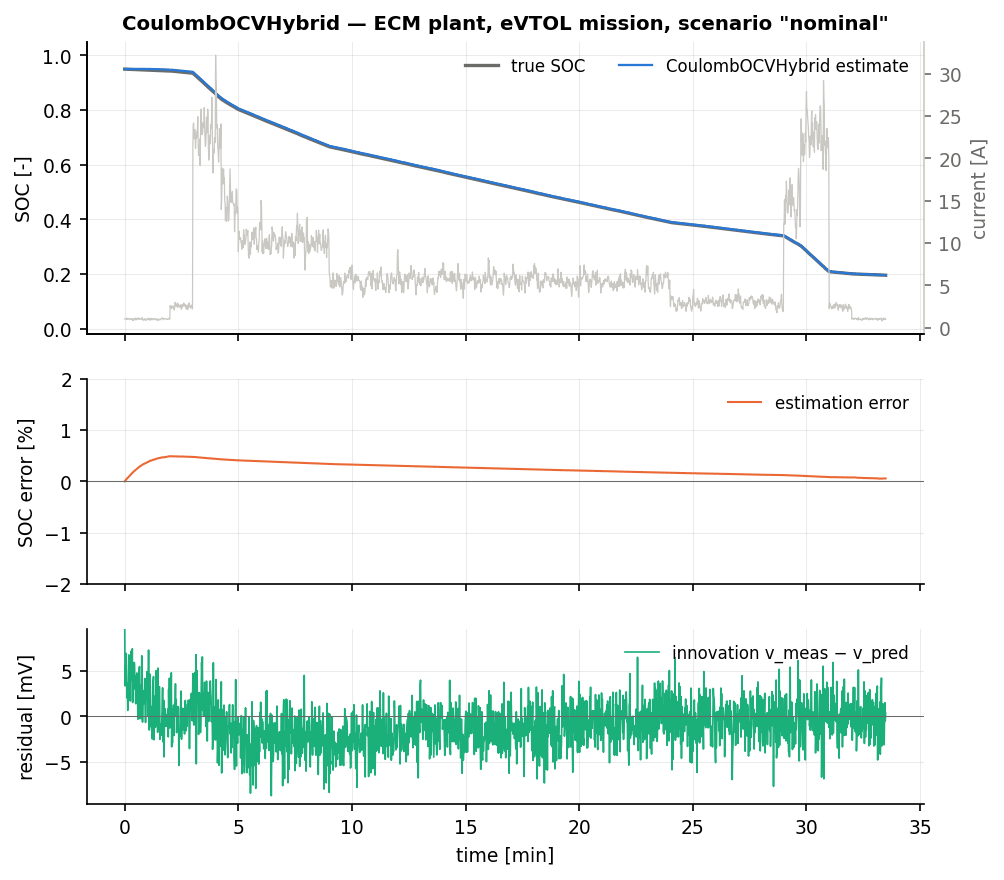
\includegraphics[width=0.78\textwidth]{figures/cell_CoulombOCVHybrid_nominal.png}
\caption{The hybrid on the nominal eVTOL mission. The error rises to $+0.47\,\%$ during the
\SI{120}{\second} preflight as the correction pulls the count towards a proxy biased by the
uninitialised hysteresis state, holds through the flight as pure Coulomb counting, and is pulled
back towards zero during the \SI{90}{\second} postflight.}
\end{figure}
\begin{figure}[H]\centering
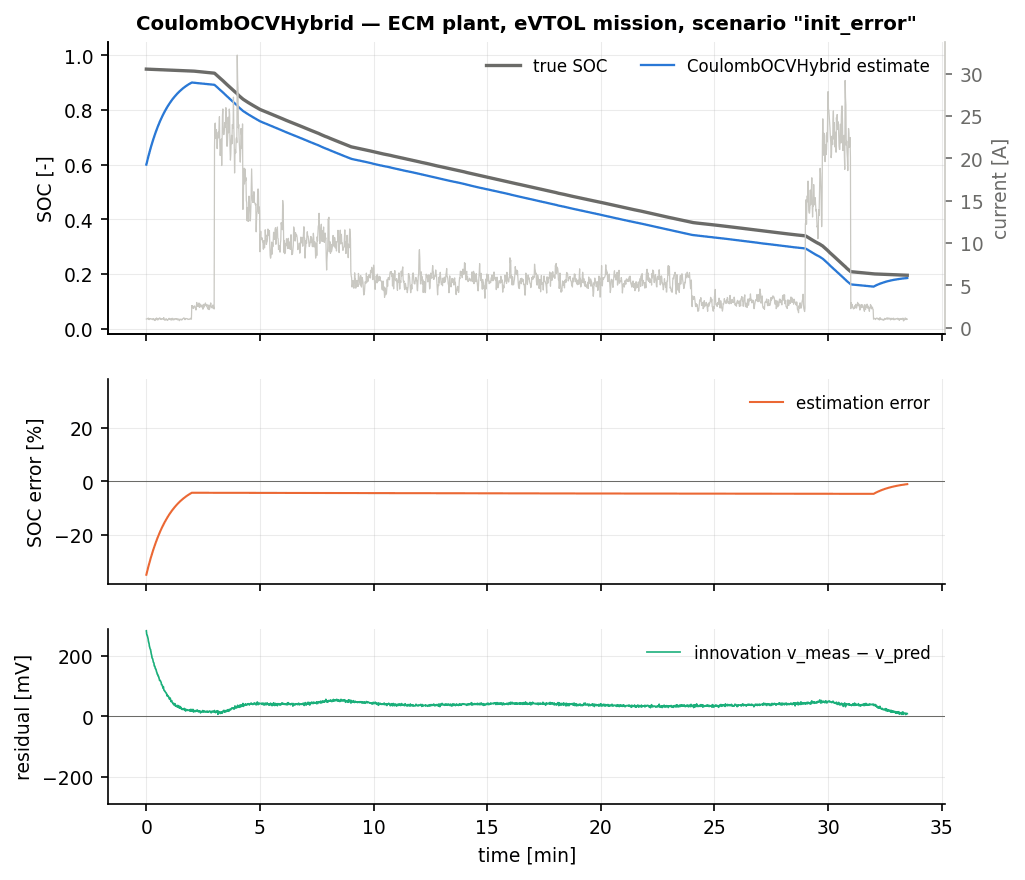
\includegraphics[width=0.78\textwidth]{figures/cell_CoulombOCVHybrid_init_error.png}
\caption{The hybrid with a $-35\,\%$ initial SOC error. Two time constants of preflight correction
contract it to $-4.4\,\%$ by $t=\SI{2}{\minute}$; the error is then frozen for the whole flight and
contracted again to about $-1\,\%$ during the postflight --- the staircase predicted by
\eqref{eq:hy-window}. Compare Chapter~\ref{ch:coulombcounting}, where the same error persists
undiminished.}
\end{figure}

\paragraph{Nominal.} $\text{RMSE}_{\text{ss}} = 0.17\,\%$ against Coulomb counting's $0.36\,\%$ and
\code{OCVLookup}'s $1.30\,\%$: the hybrid is better than either of its parents, which is the whole
point of the construction. The voltage-residual RMSE drops from \SI{3.41}{\milli\volt} to
\SI{1.79}{\milli\volt} for the same reason. The residual $0.17\,\%$ is not the Coulomb-counting
drift but the floor $e^{\ocv}$ of \eqref{eq:hy-window}: the error trace peaks at $+0.47\,\%$ during
preflight --- close to the \SI{0.6}{\percent} that a \SI{5}{\milli\volt} hysteresis bias predicts at
mid-slope --- and then decays as the drift of \eqref{eq:cc-drift}, which has the opposite sign,
works against it. Note the sign inversion relative to Coulomb counting, whose nominal error is
$-0.44\,\%$: the two methods fail in opposite directions.

\paragraph{Initial error.} $\text{RMSE}_{\text{ss}} = 4.42\,\%$ against Coulomb counting's
$35.35\,\%$, with the divergence flag cleared. Equation~\eqref{eq:hy-window} with
$T_w = \SI{120}{\second}$ predicts $35\times e^{-2} = 4.7\,\%$ surviving the preflight window, which
is what the trace holds for the rest of the flight; the postflight window contracts it by a further
$e^{-1.5} = 0.22$. The convergence criterion still reports ``--'', because the error only falls
below \SI{2}{\percent} in the final minute and never sustains it for the required
\SI{60}{\second} --- an honest reading: a $35\,\%$ prior error is \emph{survived}, not removed.

\paragraph{Faults on the current channel.} \code{current\_bias} gives $1.94\,\%$ against Coulomb
counting's $3.20\,\%$, and \code{combined} $1.33\,\%$ against $20.94\,\%$ --- a factor of sixteen,
and the largest single improvement in the baseline part. In \code{combined} the correction removes
most of the $-25\,\%$ prior during preflight and then re-anchors after the landing hover, so the
convergence criterion is met at $t=\SI{252}{\second}$ where Coulomb counting never converges. The
remaining $1.33\,\%$ is the flight-phase drift of a \SI{0.15}{\ampere} bias and a \SI{10}{\percent}
capacity error accumulating unchecked between the two windows. \code{aged\_cell} improves only
marginally ($9.41\,\%$ against $10.05\,\%$): the capacity error is a \emph{rate}, so it regenerates
during the \SI{30}{\minute} of open-loop flight faster than \SI{210}{\second} of correction can
remove it. That contrast --- a bias is removed, a rate is not --- is the sharpest statement of what
a periodically-corrected integrator can and cannot do.

\paragraph{Faults on the voltage channel.} These now matter, because the voltage is used.
\code{noise\_step} and \code{sensor\_dropout} are both unchanged from nominal at $0.17\,\%$, for the
same reason in both cases: the voltage step at $t=\SI{600}{\second}$ and the \SI{15}{\second}
dropout from $t=\SI{200}{\second}$ both fall inside high-current segments, where the correction is
switched off. The method is accidentally immune to any voltage fault that occurs in flight --- a
genuine robustness property of load gating, and a fragile one, since a fault during preflight would
be adopted directly. \code{outliers} scores $0.05\,\%$, better than nominal, because the
$\pm\SI{50}{\milli\volt}$ outliers are zero-mean, the \SI{60}{\second} correction averages them
away, and the extra noise happens to perturb the proxy against the hysteresis bias --- a coincidence
of one seed set, not a property.

\paragraph{Hysteresis.} \code{preisach} is the method's worst ECM scenario at
$\text{RMSE}_{\text{ss}} = 2.28\,\%$, against $0.36\,\%$ for Coulomb counting, which ignores the
voltage entirely, and $0.20\,\%$ for the EKF. The mechanism is \eqref{eq:hy-proxy}: the plant's
32-relay Preisach operator has a major-loop half-width of \SI{15}{\milli\volt} with the charging
branch above the discharging branch, while the estimator subtracts only $M\hat h$ with
$M = \SI{5}{\milli\volt}$ from an $\hat h$ that is itself propagated open-loop. The proxy is
therefore biased by \SIrange{15}{20}{\milli\volt}, and \eqref{eq:ocv-error} converts that to
\SIrange{1.9}{2.5}{\percent} of SOC at mid-slope. This is the characteristic failure of the whole
design: the correction is only as good as the OCV proxy, and it imports the proxy's bias with full
weight. Coulomb counting is \emph{better} here precisely because it declines to look.
\code{param\_mismatch} ($0.16\,\%$), by contrast, is essentially unaffected --- the $R_0$ and $R_1$
errors are multiplied by \SI{1}{\ampere} during the correction windows and contribute under
\SI{4}{\milli\volt}.

\paragraph{The SPM plant.} On the electrochemical plant the estimators are given a 2-RC circuit
fitted to it with a \SI{4}{\milli\volt} structured residual (Chapter~\ref{ch:spm}), and the hybrid
inherits that residual through its proxy: $\text{RMSE}_{\text{ss}} = 0.66\,\%$ on \code{nominal},
against $0.47\,\%$ for Coulomb counting and $2.03\,\%$ for \code{OCVLookup}. The ordering is the
informative part. The hybrid is \emph{worse} than pure integration, because it injects a biased
voltage estimate into an otherwise unbiased count; but it is three times \emph{better} than pure
inversion, because it only does so at \SI{1}{\ampere}, where the SPM's Butler--Volmer and diffusion
overpotentials are smallest, and because the \SI{60}{\second} correction is much shorter than
\code{OCVLookup}'s permanent \SI{30}{\second} lag applied at hover currents. The \code{cold} row
makes the same point at the limit: at \SI{-10}{\celsius} the SPM's diffusion impedance is not
representable by the fitted circuit at all, the proxy is wrong by tens of millivolts even at
\SI{1}{\ampere}, and the hybrid degrades to $3.50\,\%$ with the convergence criterion never met,
while Coulomb counting scores $0.47\,\%$. Elsewhere on the SPM plant the pattern of the ECM rows
survives: \code{current\_bias} $2.90\,\%$ improves on Coulomb counting's $3.31\,\%$,
\code{init\_error} contracts $35\,\%$ to $5.23\,\%$, and \code{hot} ($0.46\,\%$) is the best row of
all because the higher temperature both shrinks the overpotential and speeds the kinetics the fitted
circuit gets wrong. With the single exception of \code{init\_error} --- where the EKF's covariance
lets it absorb the prior error in one sample and score $3.81\,\%$ against the hybrid's $5.23\,\%$
--- every one of these rows beats the EKF's own SPM figures (\numrange{3.73}{7.35}\,\%). That is the
recurring surprise of the SPM columns: when the measurement model carries a structured error, a
method that uses the measurement sparingly does better than one that trusts it every sample.

\section{Summary}
Use load-gated OCV correction whenever the duty cycle spends even a few per cent of its time at a
fraction of the cruise current, which almost every real mission does --- it costs
\SI{211}{\nano\second} per step, removes a $35\,\%$ prior error down to $4.4\,\%$, cuts the
\code{combined} scenario by a factor of sixteen against plain Coulomb counting, and is the best of
the three baselines on seven of the twelve ECM scenarios (tied with Coulomb counting on an
eighth, \code{hot}). Size the threshold from the mission's current
staircase rather than by tuning, band it with hysteresis so that a segment sitting on the threshold
does not chatter, and choose $\tau_{\text{corr}}$ so that the shortest useful window is two or three
time constants. Do not use it where the OCV proxy is biased rather than noisy --- unmodelled
hysteresis (\code{preisach}, $2.28\,\%$) and structured electrochemical model error at low
temperature (SPM \code{cold}, $3.50\,\%$) are both imported at full weight --- and do not expect it
to track a \emph{drifting} capacity, because \code{aged\_cell} shows that a rate regenerates between
correction windows faster than the windows can remove it. Its real lesson for the rest of this
report is structural: it is a Kalman filter with the gain replaced by a hand-set schedule, and every
one of its failures is a case where a covariance would have told the estimator how much to trust the
measurement.
